\chapter{I\textsuperscript{2}C sučelje mikrokontrolera STM32L471VGT6}
Za konfiguraciju kamere Arducam 5MP Mini Plus  PDH računalo koristi
I\textsuperscript{2}C komunikaciju. S obzirom na to da se za razvoj programske
potpore PDH računala koriste \textit{Low-Layer} biblioteke, potrebno je
razumijevanje načina rada I\textsuperscript{2}C periferije odabranog
mikrokontrolera kako bi se ispravno implementirali upravljački programi. U
nastavku slijedi općenit opis I\textsuperscript{2}C komunikacije kao i njena
implementacija na STM32L471VGT6 mikrokontroleru.

\section{I\textsuperscript{2}C protokol}
I\textsuperscript{2}C (\textit{Inter-Integrated Circuit}) je jednostavna
dvosmjerna sinkrona serijska sabirnica razvijena od strane \textit{Philips
Semiconductors} (sada \textit{NXP Semiconductors}) 1982. godine. Koristi dvije
linije:
\begin{itemize}
	\item serijska podatkovna linija (SDA, \textit{Serial Data Line}),
	\item serijska taktna linija (SCL, \textit{Serial Clock Line}),
\end{itemize}
obje linije su pritegnute na visoku logičku razinu preko \textit{pull-up}
otpornika. Moguće brzine prijenosa su:
\begin{itemize}
	\item do 100 \si{kbit/s} u \textit{Standard-mode} načinu rada, 
	\item do 400 \si{kbit/s} u \textit{Fast-mode} načinu rada,
	\item do 1 \si{Mbit/s} u \textit{Fast-mode Plus} načinu rada,
	\item do 3.4 \si{Mbit/s} u \textit{High-speed} načinu rada.
\end{itemize}
Navedene brzine se koriste kod dvosmjernog prijenosa, a moguća je i brzina do 5
\si{Mbit/s} u jednosmjernom prijenosu. Više uređaja se može spojiti na jednu
sabirnicu, a svaki uređaje je prepoznatljiv po svojoj jedinstvenoj adresi i
može se ponašati kao prijamnik ili odašiljač, ovisno o funkciji uređaja.
Protokol najčešće, a tako i u ovom slučaju, koristi 7-bitno adresiranje, a
moguće je i korištenje 10-bitnog adresiranja. Uz prijamnike i odašiljače uređaj
također može biti upravljač ili meta tijekom prijenosa podataka. Upravljač je
uređaj koji inicijalizira prijenos podataka na sabirnici i generira signal
takta kako bi omogućio prijenos. U tom trenutku, bilo koji uređaj koji je
adresiran smatra se metom.

Na I\textsuperscript{2}C sabirnicu se također može spojiti više upravljača, a
primjer jednog takvog spoja sa dva mikrokontrolera je dan na sljedećoj slici.
\begin{figure}[hp]
	\centering
	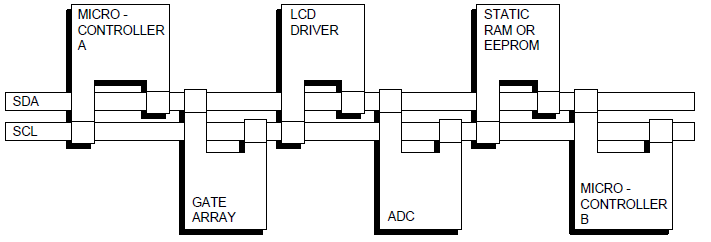
\includegraphics[width=\textwidth]{i2c_primjer_1.PNG}
	\caption{Primjer I\textsuperscript{2}C sabirnice sa spojena dva
	mikrokontrolera}
	\label{fig:i2c_primjer_1}
\end{figure}
Prijenos podataka bi možda mogao izgledati ovako:
\begin{enumerate}
	\item Mikrokontroler A želi poslati podatke mikrokontroleru B:
	\begin{itemize}
		\item mikrokontroler A (upravljač) adresira mikrokontroler B (meta)
		\item mikrokontroler A (upravljač-odašiljač) šalje podatke
		mikrokontroleru B (meta-prijamnik)
		\item mikrokontroler A prekida prijenos
	\end{itemize}
	\item Mikrokontroler A želi primiti podatke sa mikrokontrolera B:
		\begin{itemize}
		\item mikrokontroler A (upravljač) adresira mikrokontroler B (meta)
		\item mikrokontroler A (upravljač-prijamnik) prima podtke sa
		mikrokontrolera B (meta-odašiljač)
		\item mikroknotroler A prekida prijenos.
	\end{itemize}
\end{enumerate}
U svakom od navedenih slučajeva mikrokontroler A je generirao takt i prekidao
prijenos. Upravljač uvijek generira takt na I\textsuperscript{2}C sabirnici kod
prijenosa podataka. U ovom radu korišten je samo jedan mikrokontroler, odnosno
upravljač, pa ćemo se dalje usredotočiti samo na taj slučaj.